% Author: Izaak Neutelings (October 2020)
\documentclass[border=3pt,tikz]{standalone}
\usepackage{physics}
\usepackage{tikz}
\usepackage[outline]{contour} % glow around text
\usetikzlibrary{calc}
\usetikzlibrary{angles,quotes} % for pic
\usetikzlibrary{arrows.meta}
\usetikzlibrary{patterns}
\tikzset{>=latex} % for LaTeX arrow head
\contourlength{1.35pt}

\colorlet{xcol}{blue!70!black}
\colorlet{vcol}{green!60!black}
\colorlet{myred}{red!65!black}
\colorlet{mypurple}{blue!60!red!80}
\colorlet{acol}{red!50!blue!80!black!80}
\tikzstyle{rvec}=[->,xcol,very thick,line cap=round]
\tikzstyle{vvec}=[->,vcol,very thick,line cap=round]
\tikzstyle{myarr}=[{Latex[length=3,width=3]}-,xcol]
\tikzstyle{myarr2}=[{Latex[length=2,width=3]}-{Latex[length=2,width=3]}]
\tikzstyle{force}=[->,myred,very thick,line cap=round]
\tikzstyle{Fproj}=[force,myred!40]
\tikzstyle{mass}=[line width=0.6,draw=red!30!black, %rounded corners=1,
                  top color=red!40!black!30,bottom color=red!40!black!10,shading angle=30]
\tikzstyle{dark mass}=[line width=0.3,red!30!black, %rounded corners=1,
                       top color=red!40!black!40,bottom color=red!40!black!60,shading angle=30]
\tikzstyle{ground}=[preaction={fill,top color=black!10,bottom color=black!5,shading angle=20},
                    fill,pattern=north east lines,draw=none,minimum width=0.3,minimum height=0.6]
\tikzstyle{metal}=[fill,top color=black!40,bottom color=black!20,shading angle=10]
\tikzstyle{pulcol}=[draw=blue!30!black,%fill=blue!40!black!10
                    top color=blue!40!black!20,bottom color=blue!40!black!10,shading angle=20]
\tikzstyle{rope}=[brown!70!black,very thick,line cap=round]
\def\rope#1{ \draw[black,line width=1.5] #1; \draw[rope] #1; }
\tikzstyle{mount}=[blue!20!black,fill,top color=blue!20!black!70,bottom color=blue!20!black!40,shading angle=10]


\def\r{0.05} % pulley small radius
\tikzset{
  pics/Tin/.style={
    code={
      \def\R{0.12}
      \draw[pic actions,line width=0.6,#1,fill=white] % ,thick
        (0,0) circle (\R) (-135:.75*\R) -- (45:.75*\R) (-45:.75*\R) -- (135:.75*\R);
  }},
  pics/Tout/.style={
    code={
      \def\R{0.12}
      \draw[pic actions,line width=0.6,#1,fill=white] (0,0) circle (\R);
      \fill[pic actions,#1] (0,0) circle (0.3*\R);
  }},
  pics/rotarr/.style={
    code={
      \draw[white,very thick] ({#1*cos(200)},0) arc(-200:30:{#1} and {#1/2}) --++ (125:0.1);
      \draw[->] ({#1*cos(200)},0) coordinate (W1) arc(-200:20:{#1} and {#1/2}) node[midway] (W2) {} --++ (125:0.1) coordinate (W3);
  }},
  pics/pulley/.style={
    code={
      \draw[pulcol,line width=0.6] (0,0) circle (#1);
      \draw[pulcol,thick] (0,0) circle (\r);
  }},
  pics/mount/.style args={#1:#2}{ % angle, length
    code={
      \draw [mount] (0,0)++(#1-90:0.9*\r) arc (#1-90:#1-270:0.9*\r) --++ (#1:#2) --++ (#1-90:1.8*\r) -- cycle;
    }
  },
  pics/Tin/.default=mypurple,
  pics/Tout/.default=mypurple,
  pics/rotarr/.default=0.4,
  pics/pulley/.default=0.3,
}


\newcommand\rightAngle[4]{
  \pgfmathanglebetweenpoints{\pgfpointanchor{#2}{center}}{\pgfpointanchor{#3}{center}}
  \coordinate (tmpRA) at ($(#2)+(\pgfmathresult+45:#4)$);
  \draw[white,line width=0.7] ($(#2)!(tmpRA)!(#1)$) -- (tmpRA) -- ($(#2)!(tmpRA)!(#3)$);
  \draw[xcol!30!black] ($(#2)!(tmpRA)!(#1)$) -- (tmpRA) -- ($(#2)!(tmpRA)!(#3)$);
}

\begin{document}


% MOMENT OF INERTIA - mass in circle
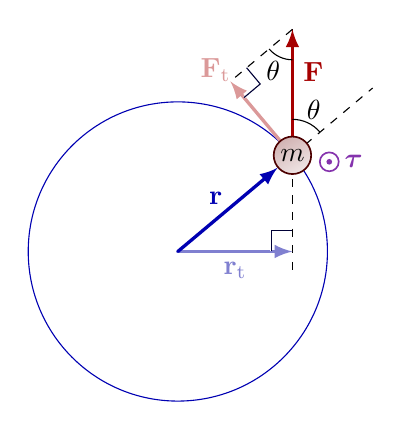
\begin{tikzpicture}
  \def\R{1.9}   % circle radius
  \def\r{1.4}   % mass radius (inner sep)
  \def\F{1.6}   % force magnitude
  \def\ang{40}  % mass anglular position
  \def\Fang{50} % force angle w.r.t. position vector
  \coordinate (O) at (0,0);
  \coordinate (R) at (\ang:\R);
  \coordinate (F) at ($(R)+(\ang+\Fang:\F)$);
  \coordinate (FT) at ($(R)+(\ang+90:{\F*sin(\Fang)})$); % perpendicular to position vector
  \coordinate (T) at ($(R)+(\ang-50:0.25*\R)$); % torque
  \coordinate (RT) at ($(R)+(\ang+\Fang-180:{\R*sin(\ang)})$);
  \draw[xcol] (O) circle(\R);
  \draw[dashed] (R) --++ (\ang:0.7*\R) coordinate (E);
  \draw[dashed] (F) -- (FT);
  \draw[dashed] (F) -- (RT) --++ (\ang+\Fang-180:0.16*\R);
  \draw[force] (R) -- (F) node[midway,above right=0] {$\vb{F}$};
  %\draw[Fproj] ([yshift=2.3,xshift=2.4]R) -- ([yshift=2.2,xshift=2.4]FT) node[above left=-4] {$\vb{F}_\mathrm{T}$};
  \draw[Fproj] (R) -- (FT) node[above left=-4] {$\vb{F}_\mathrm{t}$};
  %\draw[vvec] ([yshift=0]R) --++ (\ang+90:0.6*\F) node[below=1,left=-4] {$\vb{v}$};
  \node[mass,circle,inner sep=\r] (R') at (R) {$m$};
  \draw[rvec,xcol!90!black!50] (O) -- (RT) node[midway,below] {$\vb{r}_\mathrm{t}$};
  \draw[rvec] (O) -- (R') node[midway,above left=-2] {$\vb{r}$};
  \draw pic["$\theta$",draw,angle radius=13,angle eccentricity=1.4] {angle=E--R--F};
  \draw pic["$\theta$",draw,angle radius=11,angle eccentricity=1.5] {angle=FT--F--R};
  \rightAngle{O}{RT}{R}{0.38}
  \rightAngle{F}{FT}{R}{0.38}
  \pic[scale=1] at (T) {Tout};
  \node[mypurple,right=2] at (T) {$\vb*\tau$};
\end{tikzpicture}


% MOMENT OF INERTIA - masses on rods
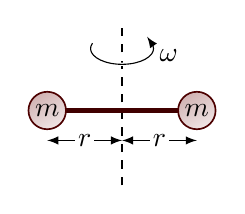
\begin{tikzpicture}
  \def\R{1.9}   % circle radius
  \def\r{1.4}   % mass radius (inner sep)
  \def\ang{40}  % mass anglular position
  \coordinate (O) at (0,0);
  \coordinate (L) at (-\R/2,0);
  \coordinate (R) at ( \R/2,0);
  \draw[dashed] (0,-0.5*\R) -- (0,0.55*\R) coordinate (T);
  \pic[scale=1] at ($(T)+(0,-0.1*\R)$) {rotarr};
  \node[below right=1] at (W3) {$\omega$};
  \draw[line width=1.8,red!25!black] (L) -- (R);
  \node[mass,circle,inner sep=\r] (L') at (L) {$m$};
  \node[mass,circle,inner sep=\r] (R') at (R) {$m$};
  \draw[<->] (L)++(0,-0.2*\R) --++ ( \R/2,0) node[midway,fill=white,inner sep=1] {$r$}; %\frac{r}{2}
  \draw[<->] (R)++(0,-0.2*\R) --++ (-\R/2,0) node[midway,fill=white,inner sep=1] {$r$};
\end{tikzpicture}


% MOMENT OF INERTIA - masses on rods - shifted
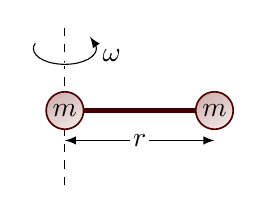
\begin{tikzpicture}
  \def\R{1.9}   % circle radius
  \def\r{1.4}   % mass radius (inner sep)
  \def\ang{40}  % mass anglular position
  \coordinate (O) at (0,0);
  \coordinate (L) at (-\R/2,0);
  \coordinate (R) at ( \R/2,0);
  \draw[dashed] (-\R/2,-0.5*\R) --++ (0,1.05*\R) coordinate (T);
  \pic[scale=1] at ($(T)+(0,-0.1*\R)$) {rotarr};
  \node[below right=1] at (W3) {$\omega$};
  \draw[line width=1.8,red!25!black] (L) -- (R);
  \node[mass,circle,inner sep=\r] (L') at (L) {$m$};
  \node[mass,circle,inner sep=\r] (R') at (R) {$m$};
  \draw[<->] (L)++(0,-0.2*\R) --++ (\R,0) node[midway,fill=white,inner sep=1] {$r$};
\end{tikzpicture}


% MOMENT OF INERTIA - masses on rods
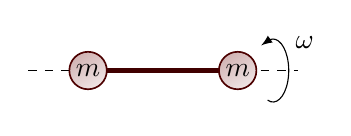
\begin{tikzpicture}
  \def\R{1.9}   % circle radius
  \def\r{1.4}   % mass radius (inner sep)
  \def\ang{40}  % mass anglular position
  \coordinate (O) at (0,0);
  \coordinate (L) at (-\R/2,0);
  \coordinate (R) at ( \R/2,0);
  \draw[dashed] (-0.9*\R,0) -- (0.9*\R,0) coordinate (T);
  \pic[scale=1,rotate=90] at ($(T)+(-0.2*\R,0)$) {rotarr};
  \node[above=10,right=-1] at (W2) {$\omega$};
  \draw[line width=1.8,red!25!black] (L) -- (R);
  \node[mass,circle,inner sep=\r] (L') at (L) {$m$};
  \node[mass,circle,inner sep=\r] (R') at (R) {$m$};
\end{tikzpicture}


% MOMENT OF INERTIA - RING 2D
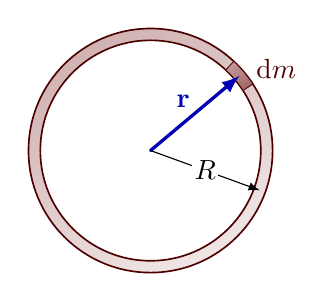
\begin{tikzpicture}
  \def\R{1.4}
  \def\dr{0.15}
  \def\ang{40}
  \def\angdr{14}
  \coordinate (O) at (0,0);
  \coordinate (R) at (\ang:\R+\dr/2);
  \draw[mass,even odd rule]
    (O) circle(\R) circle(\R+\dr);
  \draw[dark mass]
    (\ang:\R) arc(\ang:\ang+\angdr/2:\R) --++ (\ang+\angdr/2:\dr)
              arc(\ang+\angdr/2:\ang-\angdr/2:\R+\dr)
              node[midway,above=1,right=1] {$\dd{m}$} --++ (\ang-\angdr/2-180:\dr)
              arc(\ang-\angdr/2:\ang:\R);
  \draw[rvec] (O) -- (R) node[midway,above left=-2] {$\vb{r}$};
  \draw[->] (O) -- (-20:\R+\dr/2) node[midway,fill=white,inner sep=1] {$R$};
\end{tikzpicture}


% MOMENT OF INERTIA - HOLLOW CYLINDER
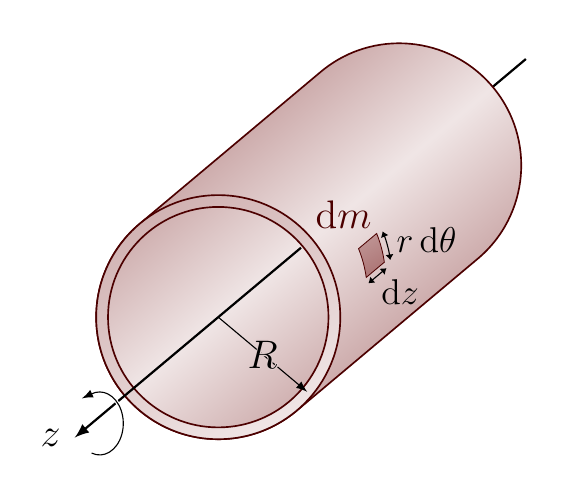
\begin{tikzpicture}
  \Large
  \def\L{3.0} % cylinder length
  \def\R{1.4}
  \def\dr{0.15}
  \def\ang{8}
  \def\angp{40} % perspective
  \def\angdr{14}
  \coordinate (O) at (0,0);
  \coordinate (R) at (\ang:\R);
  \draw[thick] (\angp:\L) --++ (\angp:1.5*\R);
  \draw[mass,
    top color=red!40!black!50,bottom color=red!40!black!50,middle color=red!40!black!10,shading angle=\angp]
    (\angp+90:\R+\dr) --++ (\angp:\L) arc(\angp+90:\angp-90:\R+\dr) --++ (\angp-180:\L) arc(\angp-90:\angp-270:\R+\dr);
  \draw[mass,even odd rule]
    (O) circle(\R) circle(\R+\dr);
  %\draw[dashed,thick] (\angp:0.98*\R) -- (\angp-180:1.7*\R);
  \draw[->,thick] (\angp:0.98*\R) -- (\angp-180:1.7*\R) node[left] {$z$};
  %\draw[dark mass]
  %  (\ang:\R) arc(\ang:\ang+\angdr/2:\R) --++ (\ang+\angdr/2:\dr)
  %            arc(\ang+\angdr/2:\ang-\angdr/2:\R+\dr)
  %            %node[midway,above=1,right=1] {$\dd{m}$}
  %            --++ (\ang-\angdr/2-180:\dr) arc(\ang-\angdr/2:\ang:\R);
  %\draw[dark mass]
  %  (\ang-\angdr/2:\R+\dr) --++ (\angp:\L) node[midway,above left=5] {$\dd{m}$}
  %  arc(\ang-\angdr/2:\ang+\angdr/2:\R+\dr) --++ (\angp-180:\L) arc(\ang+\angdr/2:\ang-\angdr/2:\R+\dr);
  \draw[dark mass]
    (\ang:\R+\dr)++(\angp:0.25*\L) coordinate (DM1) arc(\ang:\ang+\angdr:\R+\dr) node[above left=-3] {$\dd{m}$}
    --++ (\angp-180:0.1*\L) arc(\ang+\angdr:\ang:\R+\dr) -- cycle;
  \draw[myarr2] (DM1)++(-70:0.08) --++ (\angp-180:0.1*\L) node[midway,below right=-3,scale=0.9] {$\dd{z}$};
  \draw[myarr2] (DM1)++(20:0.08) arc(\ang:\ang+\angdr:\R+\dr) node[midway,above=2,right=-1,scale=0.9] {$r\dd{\theta}$};
  %\draw[rvec] (O) -- (R) node[midway,right=3,above=-1] {$\vb{r}$};
  \draw[->] (O) -- (-40:\R+\dr/2) node[midway] {\contour{red!40!black!20}{$R$}}; %,fill=red!40!black!40,inner sep=1
  \pic[xscale=1.5,rotate=90] at (\angp-180:1.5*\R) {rotarr};
  %\node[left=-1] at (W3) {$\omega$};
\end{tikzpicture}


% MOMENT OF INERTIA - DISK
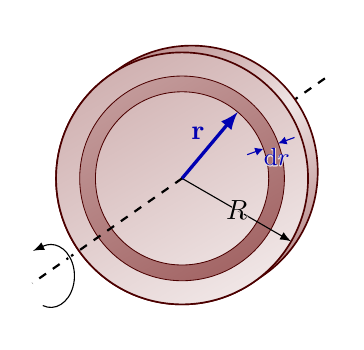
\begin{tikzpicture}
  \def\R{1.6}
  \def\r{1.1}
  \def\dr{0.2}
  \def\t{0.15} % disk thickness
  \def\angp{35} % perspective
  \def\angdr{20}
  \coordinate (O) at (0,0);
  \coordinate (R) at (50:\r);
  \coordinate (DR1) at (\angdr:\r);
  \coordinate (DR2) at (\angdr:\r+\dr);
  \draw[dashed,thick] (0,0) --++ (\angp:1.4*\R);
  \draw[mass,
    top color=red!40!black!50,bottom color=red!40!black!50,middle color=red!40!black!10,shading angle=\angp]
    (\angp+90:\R) --++ (\angp:\t) arc(\angp+90:\angp-90:\R) --++ (\angp-180:\t) arc(\angp-90:\angp-270:\R);
  \draw[mass]
    (O) circle(\R);
  \draw[dark mass,even odd rule]
    (O) circle(\r+\dr) circle(\r);
  \draw[->] (O) -- (-30:\R) node[midway] {\contour{red!40!black!15}{$R$}}; %,fill=red!40!black!13,inner sep=1
  \draw[rvec] (O) -- (R) node[midway,above left=-2] {$\vb{r}$};
  \draw[dashed,thick] (0,0) -- (\angp-180:1.45*\R);
  \draw[myarr] (DR1) node[below=3,right=-3,scale=0.9]
    {\contour{red!40!black!15}{$\dd{r}$}} --++ (\angdr-180:1.1*\dr);
  \draw[myarr] (DR2) --++ (\angdr:1.1*\dr);
  \pic[xscale=1.5,rotate=90] at (\angp-180:1.35*\R) {rotarr};
  %\node[left=-1] at (W3) {$\omega$};
\end{tikzpicture}


% DISK - PULLEY - MASS
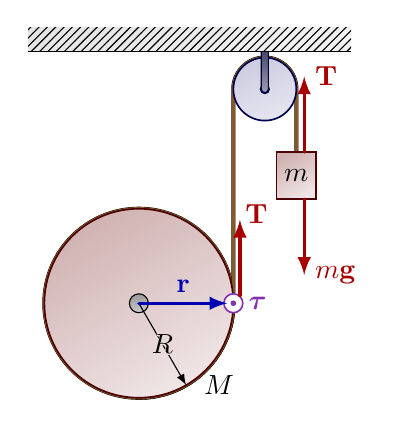
\begin{tikzpicture}
  \def\h{0.6}   % mass height
  \def\w{0.5}   % mass width
  \def\W{4.1}   % ground width
  \def\H{3.2}   % ground height
  \def\D{0.3}   % ground depth
  \def\L{0.7}   % rope length
  \def\t{0.1}   % peg thickness
  \def\R{0.40}  % pulley radius
  \def\RD{1.2}  % disk radius
  \def\px{2*\RD+\R} % pulley x position
  \def\py{0.85*\H}  % pulley y position
  \def\my{0.60*\H}  % mass y position
  \coordinate (O) at (\RD,0);      % disk origin
  \coordinate (TD) at (2*\RD,0);   % tension force on the disk
  \coordinate (P) at (\px,\py);    % pulley
  \coordinate (M) at (\px+\R,\my); % mass
  \node[inner sep=2] (TD') at (TD) {};
  
  % ROPE + PULLEY
  \rope{(2*\RD,0) arc(0:360:\RD)}
  \rope{(\RD,-\RD) arc(-90:0:\RD) -- (\px-\R,\py) arc(180:0:\R) --++ (0,\my-\py)}
  \pic at (P) {pulley={\R}};
  \pic at (P) {mount={90:\H-\py}};
  \draw[mass] (M)++(-\w/2,0) rectangle++ (\w,-\h) node[midway] {$m$};
  \draw[force] (M)++(0.1,0) --++ (0,0.8*\RD) node[right] {$\vb{T}$};
  \draw[force] (M)++(0.1,-\h) --++ (0,-0.8*\RD) node[right] {$m\vb{g}$};
  
  % GROUND
  \draw[ground] %(0,0) rectangle++ (-\D,\H) (-\D,\H) rectangle++ (\W,\D);
    (-0.05*\W,\H) rectangle++ (\W,\D);
  \draw (-0.05*\W,\H) --++ (\W,0);
  
  % DISK (FLYWHEEL)
  \draw[mass] (O) circle(\RD);
  \draw[metal] (O) circle(0.1*\RD); %node[right=2,above left=3] {$M$};
  \draw[->] (O) --++ (-60:\RD) node[midway] {\contour{red!40!black!15}{$R$}} node[right=3] {$M$};
  \pic[scale=1] at (TD) {Tout};
  \node[mypurple,right=2] at (TD) {$\vb*\tau$};
  \draw[rvec] (O) -- (TD') node[midway,above] {$\vb{r}$};
  \draw[force] (TD')++(50:0.13) --++ (0,0.8*\RD) node[above=2,right=-2] {$\vb{T}$};
  
\end{tikzpicture}


\end{document}
